% Author: Izaak Neutelings (July 2018)
\documentclass[border=3pt,tikz]{standalone}
\usepackage{amsmath}
\usepackage{tikz}
\tikzset{>=latex} % for LaTeX arrow head
%\usepackage{xcolor}
%\colorlet{charge+}{blue!80!white}
\tikzstyle{charge0}=[top color=green!80!black!50,bottom color=green!80!black,shading angle=20]
\tikzstyle{charge+}=[top color=red!50,bottom color=red!70!black,shading angle=20]
\tikzstyle{charge-}=[top color=blue!50,bottom color=blue!80,shading angle=20]
%\tikzstyle{charge+}=[thin,ball color=blue!60,shading angle=-10]
%\tikzstyle{charge-}=[thin,ball color=red!85,shading angle=-10]
%\tikzstyle{charge0}=[thin,ball color=green!80!black!80,shading angle=-10]



\def\d{0.8}
\def\R{1.0}
\def\N{{1.04*(\R+\d)}}


\begin{document}
\Large


% PROTON MODEL
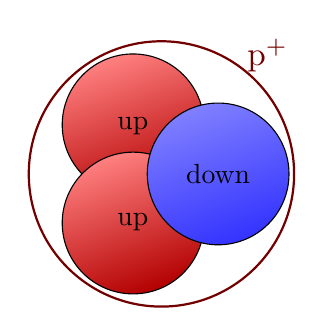
\begin{tikzpicture}[scale=0.9]

  \coordinate (O)  at (  0, 0);
  \coordinate (D1) at (  0:\d);
  \coordinate (U1) at (120:\d);
  \coordinate (U2) at (240:\d);
  \coordinate (L)  at ( 50:\N);
  
  \draw[charge+] (U1) circle (\R) node[above=2,above left=-9] {up};
  \draw[charge+] (U2) circle (\R) node[below=2,below left=-9] {up};
  \draw[charge-] (D1) circle (\R) node {down};
  \draw[thick,red!45!black] (O) circle (\N);
  \node[above right=-4,scale=1.2,red!45!black] at (L) {$\text{p}^+$};
  
\end{tikzpicture}


% NEUTRON MODEL
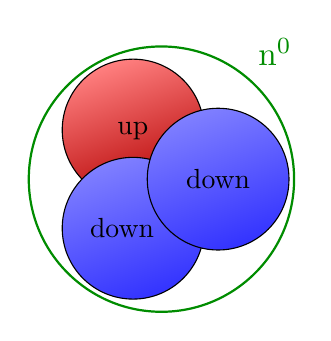
\begin{tikzpicture}[scale=0.9]
  
  \coordinate (O)  at (  0, 0);
  \coordinate (D1) at (  0:\d);
  \coordinate (D2) at (240:\d);
  \coordinate (U1) at (120:\d);
  \coordinate (L)  at ( 50:\N);
  
  \draw[charge+] (U1) circle (\R) node[above=2,above left=-9] {up};
  \draw[charge-] (D2) circle (\R) node[left=4,below=-7] {down};
  \draw[charge-] (D1) circle (\R) node {down};
  \draw[thick,green!55!black] (O) circle (\N);
  \node[above right,scale=1.2,green!55!black] at (L) {$\text{n}^0$};
  
\end{tikzpicture}


% ATOM MODEL
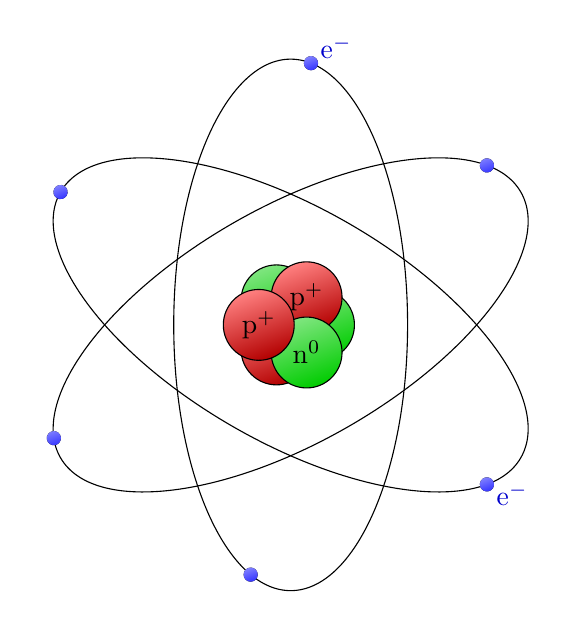
\begin{tikzpicture}[scale=0.45]
  
  \def\a{3.3}
  \def\b{7.5}
  \def\d{0.8}
  \def\D{0.9}
  \def\e{0.2} % electron radius
  
  
  \coordinate (O)  at (  0, 0);
  \coordinate (N1) at (  0:\d);
  \coordinate (N2) at (120:\d);
  \coordinate (N3) at (300:\D);
  \coordinate (P1) at (240:\d);
  \coordinate (P2) at ( 60:\D);
  \coordinate (P3) at (180:\D);
  
  % NUCLEUS
  \draw[charge0] (N1) circle (\R);
  \draw[charge0] (N2) circle (\R);
  \draw[charge+] (P1) circle (\R);
  \draw[charge+] (P2) circle (\R) node {$\text{p}^+$};
  \draw[charge0] (N3) circle (\R) node {$\text{n}^0$};
  \draw[charge+] (P3) circle (\R) node {$\text{p}^+$};
  
  % ELECTRONS
  \draw[rotate=  0] (0,0) ellipse ({\a} and {\b});
  \draw[rotate=120] (0,0) ellipse ({\a} and {\b});
  \draw[rotate=240] (0,0) ellipse ({\a} and {\b});
  \foreach \i/\ellipse/\theta [evaluate={\x=\a*cos(\theta-\ellipse); \y=\b*sin(\theta-\ellipse);}]
           in {1/0/80,2/0/250,3/120/50,4/120/200,5/240/150,6/240/-50}{
    \fill[charge-,rotate=\ellipse] (\x,\y) circle (\e) coordinate (E\i); %node[above right] {$\text{e}^-$};
  }
  
  \node[below=2,above right,blue!80!black] at (E1) {$\text{e}^-$};
  \node[below=-4,below right,blue!80!black] at (E6) {$\text{e}^-$};
  
\end{tikzpicture}


% CONDUCTION MODEL
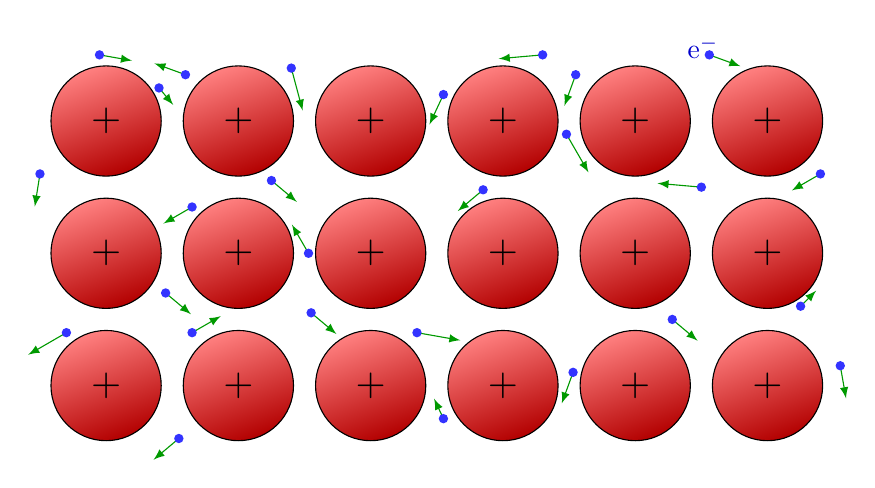
\begin{tikzpicture}[
    scale=1.4,
   %electron/.pic={
   %  \tikzset{/electron/.cd,#1}
   %  \draw[->,green!60!black] (0,0) -- (\vec);
   %  \node[circle,fill,inner sep=1.2,fill=blue!80] at (0,0,0) {};
   %}
   %/electron/.search also={/tikz},
   %/electron/.cd,
   %vec/.store in=\vec, vec={90:0.2}
   %% use as \pic at (0.20,0.90) {electron={vec={210:0.4}}};
  ]
  \def\R{0.5}
  \def\a{1.2}
  \def\Nx{6}
  \def\Ny{3}
  \def\electron#1#2#3{
    \draw[->,green!60!black] (#1*\a,#2*\a) --++ (#3);
    \node[circle,fill,inner sep=1.2,fill=blue!80] at (#1*\a,#2*\a) {};
  }
  
  % IONS
  \foreach \j in {1,...,\Ny}{ %[evaluate={\y=\j*\a;}]
    \foreach \i in {1,...,\Nx}{ %[evaluate={\x=\j*\a;}]
      \draw[charge+] ({(\i-0.5)*\a},{(\j-0.5)*\a}) circle (\R) node[scale=1.4] {$+$};
    }
  }
  
  %%%%%%%%%%%%%%%%%%%%%%%%%%%%%%% 0
  \electron{0.20}{0.90}{ 210:0.4}
  \electron{0.00}{2.10}{ -99:0.3}
  \electron{0.45}{3.00}{ -10:0.3}
  %%%%%%%%%%%%%%%%%%%%%%%%%%%%%%% 1
  \electron{1.05}{0.10}{-140:0.3}
  \electron{0.95}{1.20}{ -40:0.3}
  \electron{1.15}{0.90}{  30:0.3}
  \electron{1.15}{1.85}{ 210:0.3}
  \electron{0.90}{2.75}{ -50:0.2}
  \electron{1.10}{2.85}{ 160:0.3}
  %%%%%%%%%%%%%%%%%%%%%%%%%%%%%%% 2
  \electron{2.05}{1.05}{ -40:0.3}
  \electron{2.03}{1.50}{ 120:0.3}
  \electron{1.75}{2.05}{ -40:0.3}
  \electron{1.90}{2.90}{ -75:0.4}
  %%%%%%%%%%%%%%%%%%%%%%%%%%%%%%% 3
  \electron{3.05}{0.25}{ 115:0.2}
  \electron{2.85}{0.90}{ -10:0.4}
  \electron{3.35}{1.98}{-140:0.3}
  \electron{3.05}{2.70}{-115:0.3}
  %%%%%%%%%%%%%%%%%%%%%%%%%%%%%%% 4
  \electron{4.03}{0.60}{-110:0.3}
  \electron{3.98}{2.40}{ -60:0.4}
  \electron{3.80}{3.00}{ 185:0.4}
  \electron{4.05}{2.85}{-110:0.3}
  %%%%%%%%%%%%%%%%%%%%%%%%%%%%%%% 5
  \electron{4.78}{1.00}{ -40:0.3}
  \electron{5.00}{2.00}{ 175:0.4}
  \electron{5.06}{3.00}{ -20:0.3}
  %%%%%%%%%%%%%%%%%%%%%%%%%%%%%%% 6
  \electron{6.05}{0.65}{ -80:0.3}
  \electron{5.75}{1.10}{  45:0.2}
  \electron{5.90}{2.10}{-150:0.3}
  %%%%%%%%%%%%%%%%%%%%%%%%%%%%%%%
  
  \node[above left=-5,blue!80!black] at (5.1*\a,3.0*\a) {$\mathrm{e}^-$};
  
\end{tikzpicture}


% CUPPER ATOM
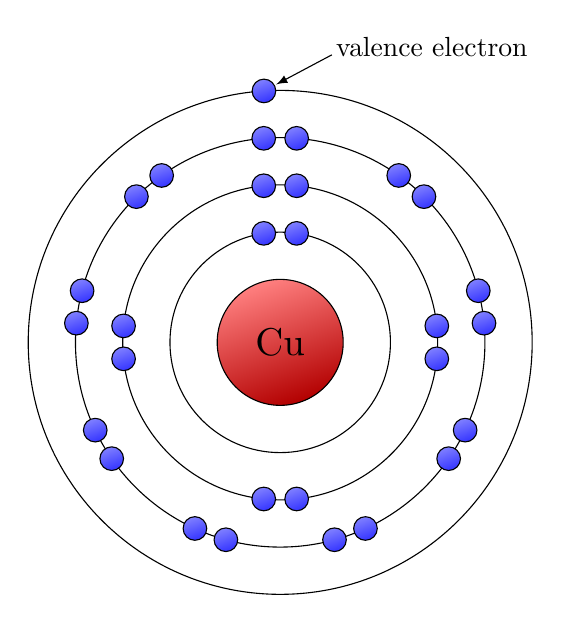
\begin{tikzpicture}
  \def\R{0.8}
  \def\a{0.6}
  \def\re{0.15}
  \def\dang{12}
  
  % NUCLEUS
  \draw[charge+] (0,0) circle (\R) node[scale=1.4] {Cu};
  
  % ORBITAL
  \foreach \i/\No [evaluate={\r=\R+\i*\a;}] in {1/1,2/4,3/9}{
    \draw (0,0) circle (\r);
    \foreach \j [evaluate={\ang=90+\j*360/\No;}] in {1,...,\No}{
      \draw[charge-] ( \dang/\r+\ang:\r) circle (\re);
      \draw[charge-] (-\dang/\r+\ang:\r) circle (\re);
    }
  }
  
  % VALENCE ELECTRON
  \draw (0,0) circle (\R+4*\a);
  \draw[charge-] (93.7:\R+4*\a) circle (\re) coordinate (V);
  \draw[<-] (V) ++ (28:1.18*\re) --++ (28:0.8) node[below=2,above right=-2] {valence electron};
  
\end{tikzpicture}


% COMPOSITE MODEL
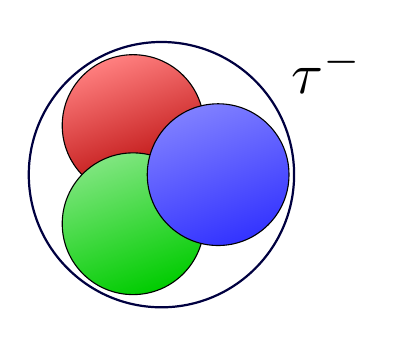
\begin{tikzpicture}[scale=0.9]

  \coordinate (O)  at (  0, 0);
  \coordinate (D1) at (  0:\d);
  \coordinate (U1) at (120:\d);
  \coordinate (U2) at (240:\d);
  \coordinate (L)  at ( 30:\N);
  
  \draw[charge+] (U1) circle (\R);
  \draw[charge0] (U2) circle (\R);
  \draw[charge-] (D1) circle (\R);
  \draw[thick,blue!25!black] (O) circle (\N);
  \node[above right=-2,scale=2.1] at (L) {$\tau^-$};
  
\end{tikzpicture}


\end{document}